\documentclass{article}
\usepackage{tikz}

\begin{document}

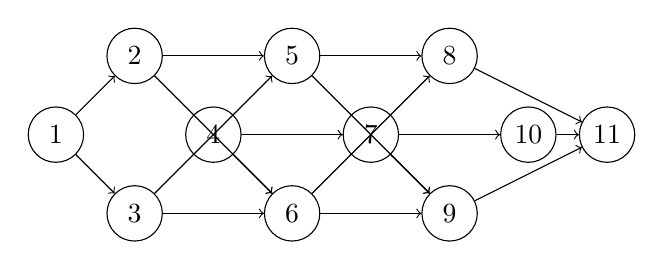
\begin{tikzpicture}[node distance=1cm]
    \tikzstyle{every node}=[draw,circle,fill=white,minimum size=20pt,inner sep=0pt]

    \node (n1) at (0,0) {1};
    \node (n2) at (1,1) {2};
    \node (n3) at (1,-1) {3};
    \node (n4) at (2,0) {4};
    \node (n5) at (3,1) {5};
    \node (n6) at (3,-1) {6};
    \node (n7) at (4,0) {7};
    \node (n8) at (5,1) {8};
    \node (n9) at (5,-1) {9};
    \node (n10) at (6,0) {10};
    \node (n11) at (7,0) {11};

    \path[->] (n1) edge (n2);
    \path[->] (n1) edge (n3);
    \path[->] (n2) edge (n5);
    \path[->] (n2) edge (n6);
    \path[->] (n3) edge (n5);
    \path[->] (n3) edge (n6);
    \path[->] (n4) edge (n6);
    \path[->] (n4) edge (n7);
    \path[->] (n5) edge (n8);
    \path[->] (n5) edge (n9);
    \path[->] (n6) edge (n8);
    \path[->] (n6) edge (n9);
    \path[->] (n7) edge (n9);
    \path[->] (n7) edge (n10);
    \path[->] (n8) edge (n11);
    \path[->] (n9) edge (n11);
    \path[->] (n10) edge (n11);
\end{tikzpicture}

\end{document}